\documentclass[a4paper]{article}
\usepackage{amsfonts}
\usepackage{amsmath}
\usepackage{amssymb}
\usepackage{graphicx}     

\begin{document}
  
\noindent \large Auteur: Thomas Eertmans \\
\noindent \large Studierichting: Informatica\\
\noindent \large Oefeningenreeks 3G nr. 9.4\\

\medskip

\normalsize

$f(x) = \dfrac{3x-8}{4-6x}$ \\

$\operatorname{dom}f: 4-6x = 0 \Leftrightarrow x = \dfrac{2}{3}$ \\

$\Rightarrow \mathbb{R}$ zonder $\dfrac{2}{3}$ \\

Nulpunten: $3x-8 = 0 \Leftrightarrow x = \dfrac{8}{3}$ \\

Verticale asymptoten: \\

$\lim\limits_{x\rightarrow\tfrac{2}{3}+} \dfrac{3x-8}{4-6x} = \dfrac{-6}{0^{(-)}} = +\infty$ \\

$\lim\limits_{x\rightarrow\tfrac{2}{3}-} \dfrac{3x-8}{4-6x} = \dfrac{-6}{0^{(+)}} = -\infty$ \\

Horizontale asymptoten: \\

$\lim\limits_{x\rightarrow+\infty} \dfrac{3x-8}{4-6x} = \dfrac{+\infty}{-\infty} \overset{\mathrm{H}}{=} -\dfrac{1}{2}$ \\

$\lim\limits_{x\rightarrow-\infty} \dfrac{3x-8}{4-6x} = \dfrac{-\infty}{+\infty} \overset{\mathrm{H}}{=} -\dfrac{1}{2}$ \\

$\Rightarrow y = -\dfrac{1}{2}$ \\

Ligging t.o.v. HA: \\

$\dfrac{3x-8}{4-6x} + \dfrac{1}{2} = \dfrac{6x-16+4-6x}{2(4-6x)} = \dfrac{-12}{2(4-6x)} = \dfrac{3}{3x-2}$ \\

\begin{tabular}{c|ccccc}
$x$ & $-\infty$ & & $\dfrac{2}{3}$ & & $+\infty$ \\ \hline
$\dfrac{3}{3x-2}$ & $0$ & $-$ & $|$ & $+$ & $0$ \\ 
\end{tabular}

Rechts van $x = \dfrac{2}{3}$ ligt de functie boven de HA en links van $x = \dfrac{2}{3}$ ligt

de functie onder de HA. \\

Geen schuine asymptoten want er zijn al horizontale asymptoten. \\

$f'(x) = \dfrac{3(4-6x)-(3x-8)(-6)}{(4-6x)^2}$ \\

$= \dfrac{12-18x+18x-48}{(4-6x)^2} = -\dfrac{36}{(4-6x)^2}$ \\

$f''(x) = -36 \cdot ((4-6x)^{-2})'$ \\

$-36 \cdot \left(\dfrac{-2}{(4-6x)^3} \cdot (4-6x)'\right)$ \\

$-36 \cdot \dfrac{12}{\left(2(2-3x)^3\right)} = -\dfrac{432}{8(2-3x)^3} = -\dfrac{54}{(2-3x)^3}$ \\

\begin{tabular}{c|cccccccc}
$x$ & $-\infty$ & & $\dfrac{2}{3}$ & & $\dfrac{8}{3}$ & & $+\infty$ \\ \hline
$f(x)$ & & $+$ & $|$ & $-$ & $0$ & $+$ \\
$f'(x)$ & & $-$ & $|^{(2)}$ & $-$ & $-$ & $-$ \\
$f''(x)$ & & $-$ & $|^{(3)}$ & $+$ & $+$ & $+$ \\ \hline
$f(x)$ & & $\searrow$ & & $\searrow$ & $\searrow$ & $\searrow$ \\
& & $\frown$ & & $\smile$ & $\smile$ & $\smile$ \\
\end{tabular}

\begin{figure}[h]
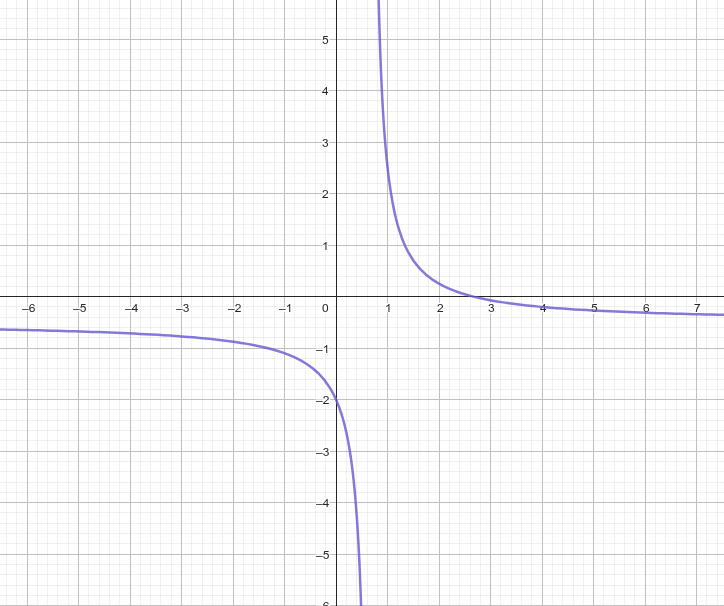
\includegraphics[width=\linewidth]{3G-9.4-thomas.eertmans.INF.png} \\
\end{figure} 
 

\begin{thebibliography}{999}
%\bibitem{a} Referentie
\end{thebibliography}
\end{document} 
